\documentclass[]{article}

%% Language and font encodings
\usepackage[english]{babel}
\usepackage[utf8x]{inputenc}
\usepackage[T1]{fontenc}

%% Sets page size and margins
\usepackage[a4paper,top=3cm,bottom=2cm,left=3cm,right=3cm,marginparwidth=1.75cm]{geometry}

%% Useful packages
\usepackage{amsmath}
\usepackage{graphicx}
\usepackage{caption}
\usepackage{subcaption}
\usepackage[colorinlistoftodos]{todonotes}
\usepackage[colorlinks=true, allcolors=blue]{hyperref}
\usepackage[linesnumbered]{algorithm2e}
\usepackage{todonotes}
\usepackage{xargs}
\newcommandx{\change}[2][1=]{\todo[linecolor=blue,backgroundcolor=blue!25,bordercolor=blue,#1]{#2}}
\usepackage{float}
\usepackage{mathtools}
\usepackage{amssymb}

\usepackage{tabularx}
\usepackage{booktabs}

\title{Playing Super Mario using Neuroevolution of Augmenting Topologies and Particle Swarm Optimization algorithms}
\author{Alex Kolmus, Christoph Schmidl, Koen Vijverberg}

\begin{document}
\maketitle
\newpage
\tableofcontents
\newpage

\begin{abstract}
In this paper we present two methods attempting to "solve" playing Mario, a game in which Mario, a plumber, must clear a level by moving right while avoiding obstacles and enemies which may harm him. A fork of the 2009 MarioAI framework with an additional Python client side is used in order to evaluate different methods. The two methods we research are: Neuroevolution of Augmenting Topologies (NEAT) and Particle swarm optimisation (PSO), in combination with Neural Networks. NEAT is a genetic algorithm which evolves artificial neural networks. The implementation is based on the neat-python package. PSO is a method that iteratively tries to optimize a problem in regards to candidate solutions (particles) inside a given search space. In the end NEAT is outperformed by the PSO algorithm in this scenario based on ambiguous environmental information given by the MarioAI framework. NEAT is not able to cope with such information based on the fact that the adjustment of weights takes a long time for correct decision making and the provided ambiguous information gives room for a significant number of local optima. PSO seems to be a promising solution here which is worth investigating. Further research could also focus on second generation PSO, also known SGPSO that could help in terms of convergence.
\end{abstract}

\section{Introduction} \label{introduction}
Computer games have always been an avenue for machine learning/artificial intelligence development due to the environment being digital, dynamic and controlled. One of the most memorable computer games of the last decades has been Super Mario. Due to the rise of AI in recent years and popularity of video games, a competition was held in 2012 in which contestants had to provide an AI which could `solve' Super Mario by beating the game\cite{karakovskiy2012mario}. 
The AIs provided by the four contestants could not beat the human `expert'. Our primary objective is not to beat human expert but to understand why a certain method works well in scenario X and utilize that knowledge to come up with an `ensemble' solution.\\

The before mentioned competition was divided into four different tracks

\begin{itemize}
    \item Gameplay track
    \item Learning track
    \item Turing Test track
    \item Level Generation track
\end{itemize}

In our case we will discard the Turing Test and Level Generation track and just concentrate on the Gameplay and Learning track. The Gameplay and Learning track are very similar to each other because their main goal is to implement an agent which clears the Super Mario game. Both tracks are using the same interface to interact with the game.\\

The main differences between these two tracks are the following:

\begin{itemize}
    \item The Gameplay track evaluates an agent's ability to clear as many levels as possible in one run
    \item The Learning track evaluates an agent's ability to clear a certain level by running through it 10000 times and using the 10001st playthrough as its final score. Agents therefore incorporate mechanisms for learning how to play a specific track.
\end{itemize}

Two different methods seemed most promising to solve this kind of problem. Neuroevolution of augmenting topologies (NEAT) and particle swarm optimization (PSO) are the main focus of this project and are discussed later on in detail.

\section{Methods} \label{Methods}

\subsection{NEAT} \label{Methods_NEAT}
Neuroevolution of augmenting topologies (NEAT), is a genetic algorithm in which a neural network evolves(both the weights and the size can alter). The algorithm was published by Stanley and Miikkulainen in 2002 \cite{stanley2002evolving} and is a frequently used to build AIs in platformers such as Super Mario. The input nodes are usually the visual cues from the screen with the output nodes being the controls.\bigskip

The genome consists of two different genes, the node genes and the connection genes. Node genes represent actual nodes in the neural network, connection genes represent the connections between nodes. All genes are assigned a so-called innovation number to enable comparison between individuals and generations.\bigskip

After assessing the fitness of each network the evolution takes place. Mutation occurs by changing the weights, or by removing/adding a node gene (and corresponding connection genes). Crossover happens by matching the two networks (using innovation numbers), the overlapping parts are averaged and the non-overlapping parts are taken from the parent with the highest fitness score. If a proper fitness function is chosen NEAT should be able to converge towards a solution.\bigskip

\begin{algorithm}[h]
\tcp{initialize population}
neural\_networks nets[P]\;
\For{population i = 1, ..., P}
{
    \tcp{draw NN weights and bias's from Gaussian with their respective parameters}
    nets[i]['weights'] = $\mathcal{N}$(weight\_mean, weight\_stddev)\;
    nets[i]['bias'] = $\mathcal{N}$(bias\_mean, bias\_stddev)\;
}
\tcp{learning steps}
\For{generation i = 1, ..., N}
{
    \tcp{evaluate every network in the population}
    \For{population j = 1, ..., P}
    {
        nets[j]['fitness'] = play\_mario(nets[i])\;
    }
    \tcp{modify neural nets with crossover/mutation and keeping the best performing $n$ networks (elitism)}
    nets = modify\_population(nets)\;
    \caption{Pseudo-code of the NEAT algorithm, the function $play\_mario$ is an abbrieviation of playing an episode of Super Mario, and receiving the score as return value. The function $modify\_population$ is, as the name suggests, a pseudo-function for modification of the networks at the end of a generation.}
}
\end{algorithm}

\subsection{PSO} \label{Methods_PSO}
Particle swarm optimization (also known as PSO) is an algorithm that attempts to find the optimum of a numerical problem by iteratively updating a group of solutions. These solutions are seen as particles and the constraints PSO puts on these particles makes them behave as a swarm, hence the name. The concept was proposed by Kennedy and Eberhart in 1995\cite{eberhart1995new} in order to simulate bird flocks, its optimization potential only became apparent later on. \medskip

The algorithm treats each particle as a separate entity and this exactly where its power lies, given enough particles (and the correct hyperparameters) PSO is able to explore and exploit the solution space. Below we show the algorithm and we will go into more detail what makes PSO such a strong optimization technique.\medskip

\begin{algorithm}[h]
    \While{termination condition}
    {    
        \For{particle i = 1, ..., S}
            {
            \tcp{determine cost of particles}
            cost[i] = eval\_cost(X[i])\;
            \BlankLine
            \BlankLine
            \tcp{update local best}
            \If{lcl\_cost[i] \textgreater cost[i]}
                {
                lcl\_cost[i] = cost[i]\;
                lcl\_best[i] = X[i]\;
                }
            }
        \BlankLine
        \BlankLine
        \tcp{update global best}
        min\_cost\_idx = argmin(cost)\;
        min\_cost = cost[min\_cost\_idx]\;
        \If{glb\_cost \textgreater min\_cost}
            {
            glb\_cost = min\_cost\;
            glb\_best = X[min\_cost\_idx]\;
            }
        \BlankLine
        \BlankLine
        \tcp{update velocities and position for all particles}
        R1 = Uniform\_rnd\_nb(0,1)\;
        R2 = Uniform\_rnd\_nb(0,1)\;
        \For{particle i = 1, ..., S}
            {
            V[i] = $\omega$ * V[i] + $\alpha_1$ * R1(lcl\_best[i] - X[i]) + $\alpha_2$ * R2 (glb\_best - X[i])\;
            X[i] = X[i] + V[i]\;
            }
    }
    \caption{particle swarm optimization, initialization is omitted, V[i] and X[i] vectors. $\omega$, $\alpha_1$ and $\alpha_2$ are hyperparameters.}
\end{algorithm}\medskip

Lets quickly go over the algorithm. Lines 2 to 8 determine the cost of the particles and whether this is the best a particle has preformed so far. Lines 9 to 14 determine whether a new global best has been found and update if needed. Lines 15 to 20 is where the magic happens, given the 3 hyperparameters $\omega$, $\alpha_1$, $\alpha_2$ the velocity (basically the displacement) and new position are calculated. These three hyperparameters determine the behaviour of the swarm, if we take a closer look at line 18 we can discern the meaning of each of these hyperparameters:
\begin{itemize}
    \item[$\omega$] It represents the previous velocity vector, so it is a momentum parameter. If $\omega$ is large the previous velocity is important, this encourages exploration of the solution space.
    \item[$\alpha_1$] It is a scalar for the difference between the particles current state and the best state the particle has been, this is the local influence. $\alpha_1$ encourage conservative behaviour and can cause pendulum movements.
    \item[$\alpha_2$] It is a scalar for the difference between the particles current state and the best observed state. $\alpha_2$ is also known as the social influence since give the particles their swarm like behaviour. 
\end{itemize}
Besides these three essential parameters one can see the random variables R1 and R2, these are there to vary the local and social influence and disrupt oscillating behaviour. \bigskip

These three hyperparameters completely control the behaviour of the swarm and thus also the effectiveness, it is crucial to obtain a (semi) optimal set of hyperparameters. The swarm can exhibit three forms of behaviour: it does not converge, it converges to a point that is not a (local) optimum, it converges to an optimum. Obviously the last option is desired so far no general method has been found to obtain the correct parameters\footnote{There are a few rules to prevent the solution from diverging, such as $\omega < 1$, and derivatives of PSO which have a dynamic $\omega$ that guarantee convergence to a local optima. However there is no method yet that guarantees finding a global optimum.}.\bigskip

\subsection{Related work}
Although back-propagation is the de facto method for updating the weights in neural network, there is at least one viable alternative updating the weights by using PSO\cite{hara2013neuroevolution, adhikari2013pso}. In the two cited articles the weights and biases are represented as the position vector and the velocity is the weight and bias update. The update rules of regular PSO apply, the velocity is updated with a combination of the current velocity, the best global velocity and the best local velocity.\bigskip

It was noted in the articles that the PSO variant had several advantages and disadvantages when compared to regular back-propagation neural networks. Due to the exploration and large number of neural networks they tend to generalize better (and since the exploitation is weak, they do not overfit), however this is only true for small networks\footnote{The solution space is very large and the number of particles needed is simply too large and finding a viable solution is basically a gamble.}. Furthermore it is applicable in cases where back-propagation cannot go\footnote{As is the case for the marioai competition, since there is no ground truth.}, due to the problem being described by a fitness function instead of ground truth values. The biggest problem PSO faces is depth, due to the large state space and the velocity updating does not work well with creating abstractions in deeper layers. Lastly, PSO appeared to be very robust with respect to initialization of the particles given a sufficient amount of particles. 

\section{Implementation}
\subsection{Framework}
\label{sec:framework}
\begin{figure*}[h]
\centering
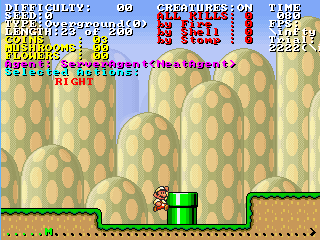
\includegraphics[width=8cm]{images/mario-screenshot.png}
\caption{A screenshot of the NEAT-agent attempting to clear a level.}
\label{fig:mario-screenshot}
\end{figure*}

The used MarioAI Framework is a fork of the 2009 MarioAI with some additions to the Python client (see: \url{https://github.com/renatopp/marioai}). The original code of the Framework was written by Sergey Karakovskiy and Julian Togelius and was targeted towards the Java programming language (see: \url{http://julian.togelius.com/mariocompetition2009/}).\\
The used framework is divided into two parts, nameley a client side which can be used to implement so called "Agents" in Python and a server side which is implemented in Java and provides the client with an environment to interact with. Although it is possible to write Agents in Java and drop the client side completely, we decided to implement our solutions with Python based on the vast majority of libraries available and personal preference/experience. Furthermore, Python seems to be a better tool for fast prototyping based on the fact that it is an interpreted language in contrast to Java which has to be compiled.\\


\begin{figure}[h]
    \centering
    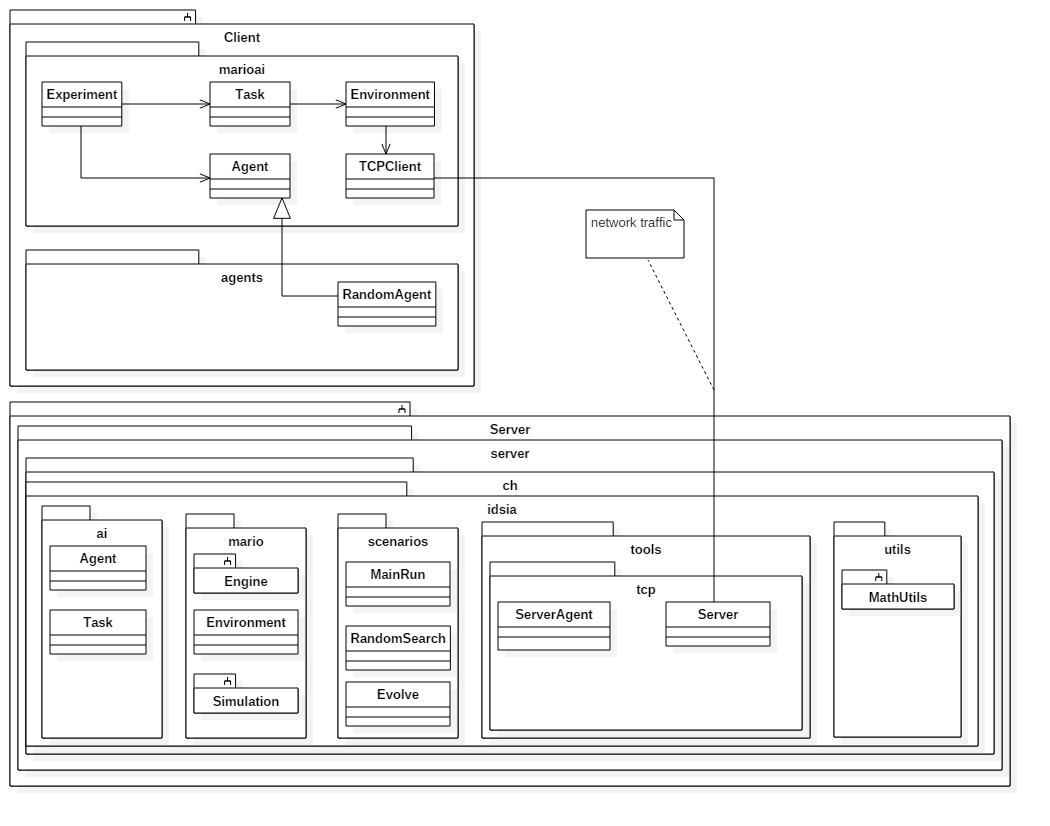
\includegraphics[width=0.9\linewidth]{images/client_server_interaction.png}
    \caption{Client-Server Interaction}
    \label{fig:client_server_interaction}
\end{figure}


The client side provides some classes which can be used as a template for one's own implementation or can be used to inherit from in order to implement an Agent. Figure~\ref{fig:client_server_interaction} provides a rough overview of the interaction between client and server side. The Experiment class can be used as the main entry point in order to implement a custom solution to the MarioAI competition.  The Experiment class' responsibility is to run different episodes which are composed of single steps. Each step provides the Agent with environmental information which it receives from the task that the Agent has to fulfill. At the end of each step a reward is returned based on the evaluation of the Task class. The Task class decides how to evaluate the observations, potentially returning reinforcement rewards or fitness values. Furthermore it is a filter for what should be visible to the agent. Also, it can potentially act as a filter on how actions are transmitted to the environment. The environment class uses the TCPClient class to connect to the running Java server. The environment class acts as the main interface from the client to the server side. It receives observations from the server which then can be forwarded to the task and is able to send actions back to the server which were generated by the Agent. Observations or so-called "sensorial information" are divided into boolean values like "can\_jump" or "on\_ground". Actions or so-called "control signals" are arrays which represent different boolean values like "backward, forward, crouch, jump, speed/bombs". The Python Agent on the client side is therefore able to interact with the environment on the server side through a TCP connection. The user can witness the Agent's influence on the game environment in real-time by a graphical representation of the game state as seen in figure~\ref{fig:mario-screenshot}.


\begin{figure}[h]
    \centering
    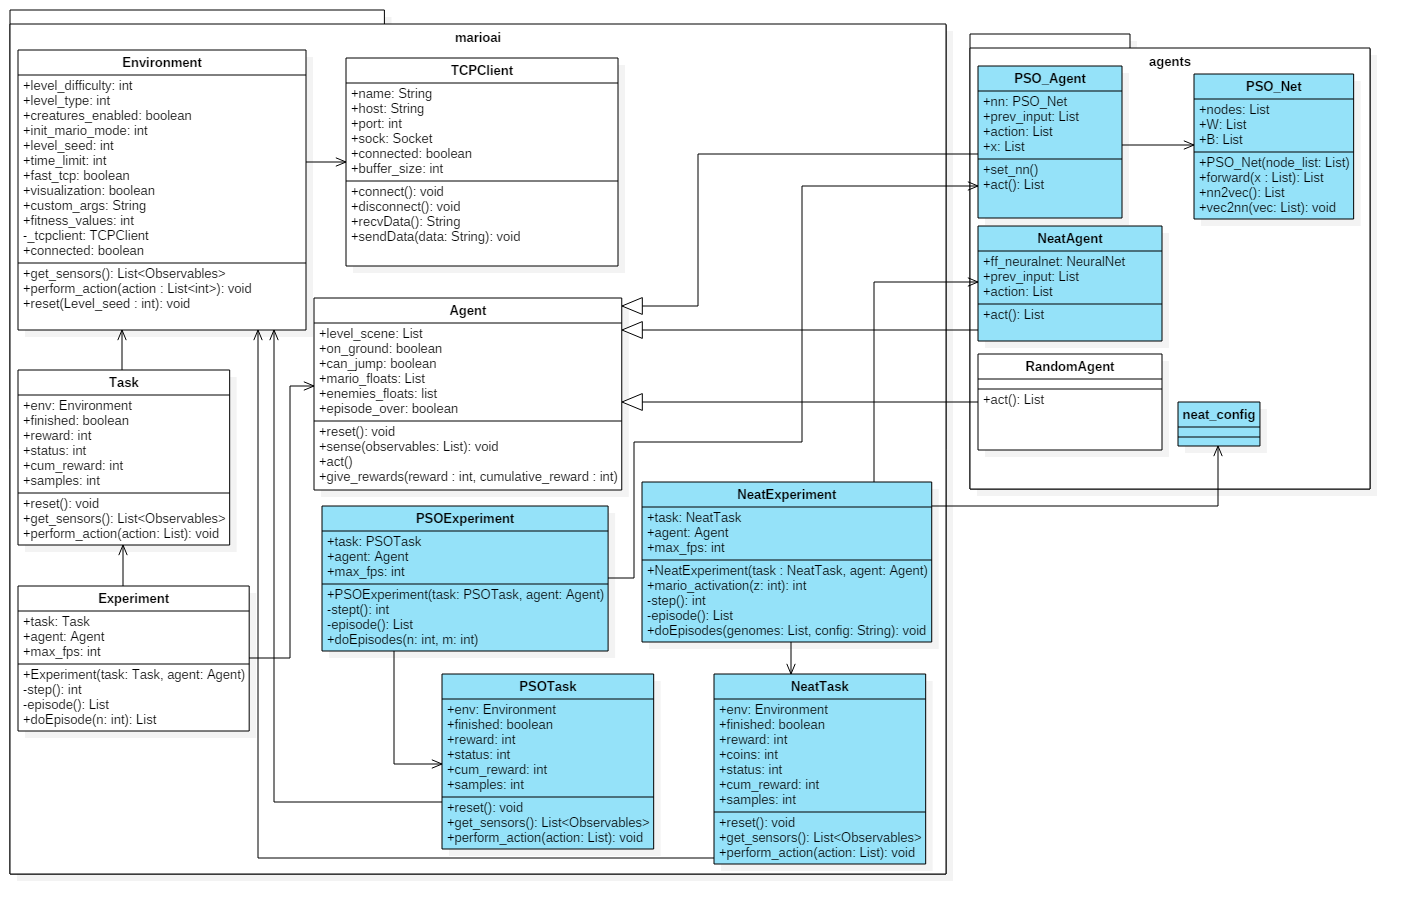
\includegraphics[width=1.0\linewidth]{images/client_side_uml.png}
    \caption{Client Side Implementation}
    \label{fig:client_side_uml}
\end{figure}


The actual implementations of NEAT and PSO have been incorporated into the given structure of the client side of the framework. Therefore the Experiment, Task and Agent classes have been copied and altered respectively. Figure~\ref{fig:client_side_uml} gives a more in-depth representation of the structure. Classes which have been marked by a coloured background are our custom implementations of PSO and NEAT while classes which have a white background are default parts of the framework. 



\subsection{NEAT}
The NEAT implementation is based on a python package called \emph{neat-python}\footnote{\url{http://neat-python.readthedocs.io/en/latest/}}. This framework allows for easy setup of most hyperparameters of NEAT. The most important hyperparameters are listed here, a few l
\begin{itemize}
    \item Neural network parameters:
    \begin{itemize}
        \item Bias mean/std 
        \item Weight mean/std: For both the bias and weights we chose mean 0 and a small stddev, since the mario's "vision" is a matrix with values -1, 0 or 1
        \item \#. of hidden units: Since Mario is not an extremely complicated we set the number of hidden units to a relatively low amount: 20 units.
    \end{itemize}
    \item Evolution parameters:
    \begin{itemize}
        \item Population size: we chose 150 as population count, a decent amount to get some variation in the population during the first (and subsequent) generation(s).
        \item Generations: we ran the experiment for 300 generations, a pretty high number, mostly because we hoped that NEAT could escape the local optimum it was in after 5 generations.
    \end{itemize}
\end{itemize}

\subsection{PSO}
We made our own implementation of PSO, which consisted of a simple neural network class and an implementation of the PSO algorithm inside the marioai environment. Below we shortly discuss the neural network structure and why we choose our hyperparameters.
\begin{itemize}
    \item The neural network is a 2-layer network, the feed-forward function is the hyperbolic tangent, it has 30 inputs (a 7 by 4 grid around Mario and two booleans that indicate whether Mario can jump and if he is on the ground). We noticed that a larger input grid would only lead to longer run times, since the number of particles that were needed to find a viable solution increased enormously with the number of inputs. There were the standard 5 outputs ('left', 'right', 'down', 'up', 'speed').
    \item The hyperparameters were chosen to be $\omega = 0.3$, $\alpha = 1.5$, this was based on a grid search, see the result section.
    \item The number of particles was set at 400, since PSO needs at least a few capable particles to obtain viable solutions.
\end{itemize}


\section{Results}
In figure \ref{fig:neat_fitness}, we can see the fitness graph of the NEAT algorithm. Unfortunately the algorithm does not learn anything new after the third generation, we ran the experiment up until the 300\textsuperscript{th} generation in the hopes of eventual improvements, since NEAT picked up how to jump Mario, which is kind of tricky in our framework (more on this in the discussion in section \ref{sec:discussion}). We tried different parameter settings of the NN weights and bias's, but converging on the right solution with NEAT (in reasonable time) seems to be quite tricky. The NEAT algorithm has a lot of parameters, with some having a substantial search space, so just brute-forcing the optimal parameters is -unlike PSO- not possible with NEAT.
\begin{figure}[h]
    \centering
    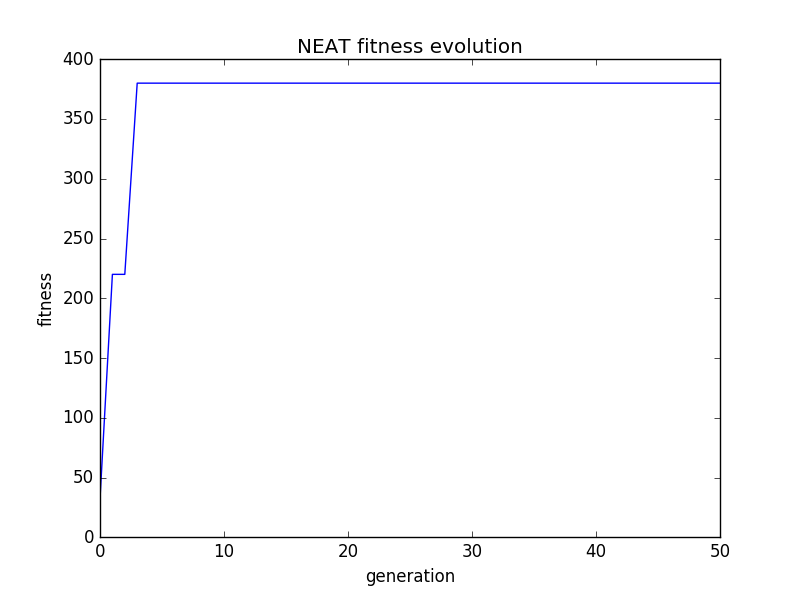
\includegraphics[width=0.8\linewidth]{images/neat_fitness.png}
    \caption{Fitness of the best Neural Network of NEAT vs the generation number.}
    \label{fig:neat_fitness}
\end{figure} \medskip

In figure \ref{fig:gridsearch} we can see the contour plots of the average(left) and global(right) reward as a function of the hyperparameters $\omega$ and $\alpha$\footnote{We have set $\alpha_1$ and $\alpha_2$ equal to each other}, light green indicates high rewards whereas dark blue represents low rewards. The contour plots are based on a grid, the vertical axis represents $\alpha$ and has a step size of 0.25 between 0 and 2, the horizontal axis represents $\omega$ and has a step size of 0.2 between 0 and 1. Since each point in the grid is only the average of two simulations\footnote{Due to time constraints we could not do more. Each grid point had 2 simulations with 5 iterations and 200 particles, which took 15 hours.} it is not truly representative, but more of an estimation. \bigskip

From these two estimations we can deduce that low $\alpha$ is undesirable. This is to be expected, since the particles have weak to no interaction with one and another they do not improve through iteration and simply stay where they are. The other observation is that high $\omega$ increases the probability of obtaining strong global rewards, we suspect that is mostly due to 'viable' solutions moving more quickly into the correct direction than anything else\footnote{Since the frequency of good global solutions is to the right, but not all good solutions are to the right. Moreover we only did 5 iterations, so high momentum and a good solution are favored.}.\bigskip

In figure \ref{fig:generation_pso} the global reward (blue) and average reward (orange) are shown as a function of the number of iterations, the vertical lines represent error bars and their length is equal to 1 standard deviation. The plot was made by averaging over 5 runs with 200 particles, $\omega =0.5$, $\alpha =1.5$ and 10 iterations. Both the global and average reward tend to increase as the number of iterations increases. However the error bars also become larger as the number of iterations increase. We attribute this to the starting values of the particles, which have a greater impact than desired due to there being \textit{only} 200.\footnote{Having enough particles would have made the running time of the script longer than 3 days which was undesirable in the latest stages of the project.} To illustrate the difference in convergence, the best run out of the 5 had solved the level (global reward = 2340) within 6 iterations and the final average reward was 1360. The worst run out of the 5 had global reward of 550 after 10 iterations and the average reward was 350. Nonetheless the results seem promising, the global and average reward increases (in general) as the iterations increase and out of the 5 runs, 2 completed the level and only 1 did poorly. Given enough particles PSO should be able to solve the level.

\begin{figure}[h]
    \centering
    \begin{subfigure}[b]{0.4\textwidth}
        \centering
        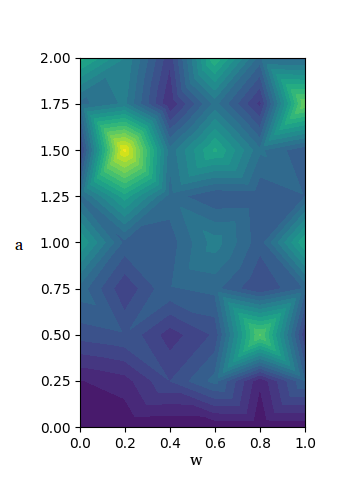
\includegraphics[width=\textwidth]{images/200_avg_results_best.png}
        \caption{The average best result.}
        \label{fig:average best}
    \end{subfigure}
    \qquad
    \begin{subfigure}[b]{0.4\textwidth}
        \centering
        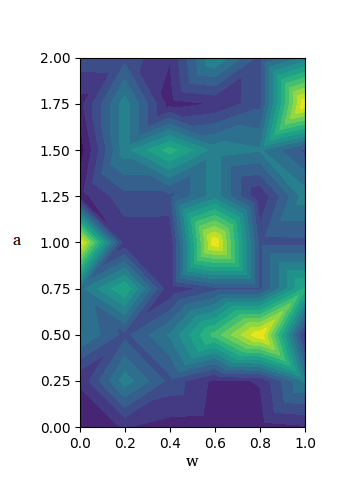
\includegraphics[width=\textwidth]{images/200_gl_results_best.png}
        \caption{The global best result}
        \label{fig:global best}
    \end{subfigure}
    \caption{Two (interpolated) contour plots, where the contour is based on the average reward(left) or global reward(right) and the vertical axis is represented by the $\alpha$ hyperparameter and the horizontal axis is the $\omega$ parameter. The contour is based on an grid with step-size 0.2 in the $\omega$ direction from 0 to 1 and step-size 0.25 in the $\alpha$ direction from 0 to 2.}
    \label{fig:gridsearch}
\end{figure}

\begin{figure}[h]
    \centering
    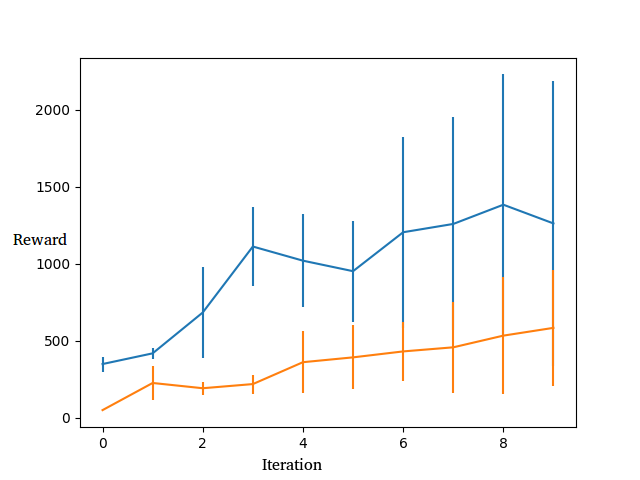
\includegraphics[width=0.75\linewidth]{images/avg_glb_gen.png}
    \caption{The reward of the best particle(blue) or the average particle(orange) as a function of the generation. The vertical bars of represent the standard deviation. The lines are made by averaging over 5 runs with 200 particles, $\omega = 0.5$, $\alpha = 1.5$ and 10 iterations. The maximum reward is 2340, which was achieved by 2 of the 5 runs. In general the global reward and average reward increase as the number of iterations increases, which shows that PSO is creating solutions that become progressively better at solving the level. The error bars increase as the number of iterations increases, this is most likely due to the individual runs not having enough particles to properly explore the solution space and thus being stuck in a local minimum.}
    \label{fig:generation_pso}
\end{figure}


\section{Discussion}
\label{sec:discussion}
The goal of this research was to compare the NEAT and PSO algorithms, since PSO achieves a higher score, PSO is the obvious winner. As to why NEAT didn't perform that well we can only make an educated guess. We think the main reason why NEAT performed sub-optimal, is that the algorithm takes a long time to select the right weights to make a correct decision. Selecting these right parameters is also hindered by the framework in multiple ways, it provides an incorrect parameter $can\_jump$, which evaluates to $False$ if Mario is in the air, while in fact he needs to keep jumping to make it across a high obstacle. Another problem is that a framework needs to figure out that Mario needs to release the jump button once he is high enough, because continuously pressing the jump button does not lead to multiple jumps. The last significant problem we encountered is that if Mario sprints into a wall he reaches a higher distance (and fitness) than if he walks (without sprinting) into that very same wall. These things combined account for a significant number of local optima, which require a high exploration rate to escape, but in turn impact the exploitation/convergence time negatively. Due to PSO performing better we invested more time in optimizing PSO hyperparameters and performance, which -in part- also impacts the NEAT performance.
\newpage

\section{Conclusion and future work}
Our implementation of NEAT was not able to complete a large part of the level, due to this we could not make a comparison between NEAT and PSO. We therefore focused more on PSO and trying to get it to work/optimize it.\bigskip

So PSO has shown to be able to complete the simple marioai level, so there is potential that it is capable to generalize to multiple mario levels or at least solve all of them by learning. The following are ideas that might prove to be helpful:
\begin{itemize}
    \item Experiment with more particles, most of the results concerning PSO are uncertain due to the large variance in results. Having particles should remove or at least reduce these issues. The only consideration should be time, doubling the number of particles, doubles the time spend. By our estimate 500 particles should be sufficient, which would multiply computing by a factor of 2.5 compared to our current work.
    \item Having $\alpha_1 \neq \alpha_2$, since the solution space is so incredibly large we suspect that following the global best a little more than then the local best should improve the convergence of the population, which was kinda troublesome in our simulations.
    \item Using second generation PSO, also known as SGPSO, we stumbled too late across this method during our project. We suspect that should help with convergence, although it does add an extra hyperparameter.
    \item Try a smaller grid window as input, one of the possible problems is that the networks `remember' how to do a track instead of learning how to jump over certain obstacles. Even though our current grid window is not big, we did not test what size is optimal/sufficient.
    \item Exclude `left' and/or `down' as an input, we noticed that excluding the left and down option improved convergence since the making correct choices was easier this way. For the sake of fairness we used all outputs, but it reduced the convergence.
\end{itemize}


\clearpage
\appendix
\section{How to run the program.}
Clone our repo: \url{https://github.com/ChristophSchmidl/marioai}

Requirements:
\begin{itemize}
    \item Java for the server
    \item Python 2.7 for the agent
    \item Python packages:
    \begin{itemize}
        \item numpy
        \item neat-python
        \item graphviz
        \item matplotlib
    \end{itemize}
\end{itemize}

Running our implementations:
\begin{enumerate}
    \item Start the server
    \begin{enumerate}
        \item On Windows: run server.bat
        \item On linux: \\
        \begin{emph}
            cd server \\
            java ch.idsia.scenarios.MainRun -server on
        \end{emph}
    \end{enumerate}
    \item Execute the python script \textit{run\_pso.py} or \textit{run\_neat.py}
    \item It should run, in figure \ref{fig:runpso} you can see the terminal output.  
\end{enumerate}

\begin{figure}[h]
    \centering
    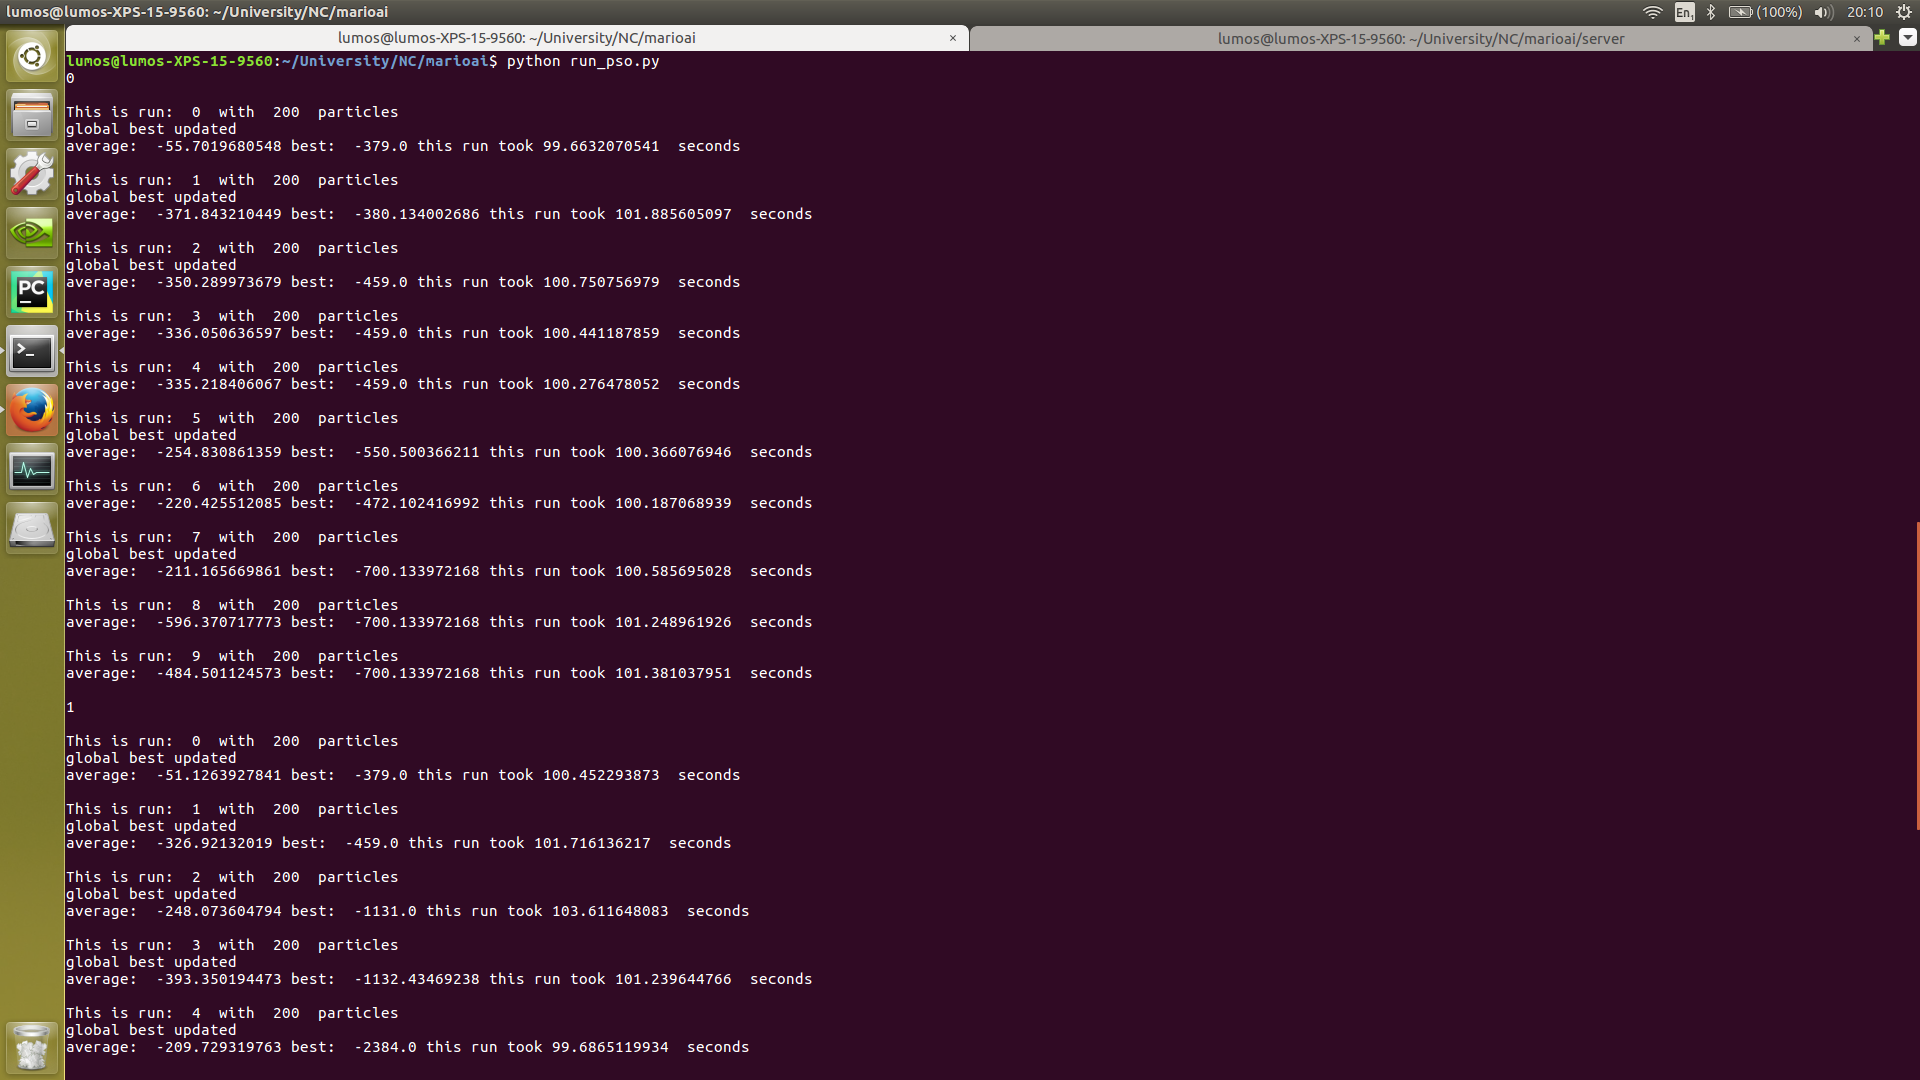
\includegraphics[width=0.8\linewidth]{images/Screenshot from 2017-06-27 20-10-29.png}
    \caption{A screenshot from the terminal when running run\_pso.py.}
    \label{fig:runpso}
\end{figure}


\section{Self reflection}
\subsection{Alex}
My contribution to the project is the PSO part. If I reflect back on the work I did for PSO, I should have spend less time on finding the `perfect' hyperparameters, since that took way too much time while I still have not found them. Everything else with the project went nicely. Within the team everything ran quite smoothly, everybody did what they said they would do and the division of work was fair.

\subsection{Christoph}

Unfortunately I was not able to contribute that much to the implementation as much as Alex and Koen did for this last project. Based on the fact that it would not have made much sense to divide the implementation parts of PSO and NEAT over more than two people, I did literature research, investigated the main structure of the MarioAI framework and where to hook in one's own implementations. Although I did some prototyping with some basic Agents and tested different approaches to test the actual usability and feasibility of the framework beforehand, the main implementation parts were done by Alex and Koen.  We had weekly meetings where we discussed our findings regarding useful papers or progression in regards to implementations. In my opinion the whole team worked nicely together, let it be the assignments or the final project. In a retrospective view it would have been nice if I could have contributed more to the main implementation instead of investigating the framework and do simple prototyping as in section \ref{sec:framework} but overall the work has been divided equally and fair during the whole course. 


\subsection{Koen}
As a team we worked quite well together, my contribution to the project were mainly the NEAT parts, which unfortunately did not perform that well, but at least we could reason why not. I also modified the Agent's way of influencing the Environment (see sec. \ref{sec:framework}), to enable it to hide the Java view (performance) and set different level seeds to generate new levels, both of which were luckily already supported on the server side. \medskip

In the course Natural Computing as a whole we also worked together quite nicely in my opinion, dividing up the work went smoothly and was performed by everyone on time. I realized that Alex and Christoph had to do more work on assignments 3\&4 due to our split of assignments, so I did assignment 5 alone to balance things out.
\bibliographystyle{ieeetr}
\bibliography{references}

\end{document}